\chapter{Methods}
\label{ch:methods}

Building on a physical background, this chapter first introduces generally applicable methods for the translation of an
injected proton distribution to a hadronic spectrum, which then decays to create neutrinos. Subsequently, the injection
spectra are decribed for the previously specified astrophysical settings. To start with, a general case $a \rightarrow b$
is defined for the reaction. Given a spectrum $dN_a \kern+0.5pt / \kern-0.25pt dE_a$ that describes the number $N_a$ of
particles $a$ per $E_a$ energy interval, as well as the spectral distribution $F_{a \rightarrow b}$ for the probability
that particles $b$ are produced by a singular interaction, one can solve the folding integral
\begin{equation}
	\frac{dN_b}{\raisebox{0.5ex}{$dE_b$}} (E_b) \kern+0.5pt = \kern-1.5pt\int_{\check{E}_a}^{\hat{E}_a} dE_a
	\kern+0.5pt \frac{dN_a}{\raisebox{0.5ex}{$dE_a$}} (E_a) \kern+1.5pt F_{a \rightarrow b} (E_b \kern+0.5pt, \kern-0.5pt E_a)
	\label{eqn:folding}
\end{equation}
to obtain their numbers $N_b$ with respect to $E_b$ energies. From this formulation, it is clear that both distributions
and spectra should be assumed to depend on energy, with other arguments such as the time $t \kern+0.5pt$ being allowed as
well. Additionally, integration bounds $\check{E}_a \leq \hat{E}_a$ must always be specified, which are usually dictated by
kinematic constraints.

To implement and compute all following parametrizations, the \emph{Python} programming language and its library \emph{Numpy}
are used. Graphical results are created via the \emph{Matplotlib} package.\footnote{$\,$In service of reproducability, all
implementations can be viewed in \href{https://github.com/fritzali/bachelor}{this} repository.}


\section{Cross Sections}
\label{sec:cross}

By defining an effective area perpendicular to the momentum vectors of projectiles and targets, cross sections as described
by section \ref{sub:collisions} measure probabilities of collision processes in particle physics and are therefore required
for the calculation of spectral distributions. 



\subsection{Scattering}
\label{sub:scattering}

To model total cross sections in hadron-proton scattering, this work uses the formula
\begin{equation}
	\sigma_{hp} = H_h \ln^2 \bigl( s \kern+1.0pt / s_h \bigr) + P_h +
	R_h^1 \bigl( s_h \kern+0.5pt / s \bigr)^{\eta_1} + R_h^2 \bigl( s_h \kern+0.5pt / s \bigr)^{\eta_2}
	\label{eqn:hpr1r2}
\end{equation}
as given in \cite{Belousov_2016} for a universal analytic parametrization of the corresponding amplitudes.

All adjustable parameters are listed in table~\ref{tab:hadron-scattering} together with relevant meson lifetimes for
cooling. In this approach, the variable $M$ \kern+0.5pt relates to $H \kern+0.5pt = \pi (\hbar c / M)^2$ and
$s_h \kern-0.5pt = (m_h + m_p + M)^2$ as an effective mass. Coefficients in \eqref{eqn:hpr1r2} are named after Heisenberg,
Pomeranchuk and Regge, respectively, and have some qualitative motivation, though the formula itself is primarily a quantitative
result.

\begin{table}[H]
	\centering
	\caption[Fits to the total cross sections in hadron proton collisions.]{Fits to the total inclusive scattering cross sections
			 in hadron proton collisions. Parameters are taken from \cite{Belousov_2016} with $M = \qty{2.121}{\giga\electronvolt}$
			 for $H = \qty{0.272}{\milli\barn}$ as the rate of growth. Both $\eta_1 = \num{0.447}$ and $\eta_2 = \num{0.5486}$ are
			 dimensionless exponents. Rest masses $m_h$ can be found in the particle listings \cite{pdg} and are given in natural units.}
	\label{tab:hadron-scattering}
	\sisetup{group-digits=integer, table-format=2.2}
	\begin{tabular}{c S S S[table-format=1.3] S[table-format=1.3] S}
		\midrule\midrule
		{$h$} & {$P_h \mathbin{/} \unit{\milli\barn}$} &
		{$R_h^1  \mathbin{/} \unit{\milli\barn}$} & {$R_h^2  \mathbin{/} \unit{\milli\barn}$} &
		{$m_h \mathbin{/} \unit{\giga\electronvolt}$} & {$s_h \mathbin{/} \unit{\giga\electronvolt\squared}$} \\
		\midrule
		{$p$} & 34.41 & 13.07 & 7.39 & 0.938 & 15.98 \\
		{$\pi$} & 18.75 & 9.56 & 1.767 & 0.140 & 10.23 \\
		{$K$} & 16.36 & 4.29 & 3.408 & 0.494 & 12.62 \\
		\midrule\midrule
	\end{tabular}
\end{table}


Assuming a quasi universal ratio $\mathscr{R}$ between elastic and total hadron cross sections, one obtains the inelastic
cross section $\sigma_\text{inel} = (1 - \mathscr{R}) \sigma_\text{tot}$ from $\sigma_\text{el} = \mathscr{R} \sigma_\text{tot}$
and $\sigma_\text{el} + \sigma_\text{inel} = \sigma_\text{tot}$ as a unitarity condition. Provided in \cite{Fagundes_2012} is
the model independent parametrization
\begin{equation}
	\mathscr{R}(s) = \frac{\sigma_{\text{el}\kern+0.5pt} (s)}{\sigma_{\text{tot}\kern+0.5pt} (s)} =
	\mathscr{A} \tanh \bigl( \kern+1.0pt \gamma_1 \kern-1.0pt - \gamma_2 \ln (s) + \gamma_3 \ln^2 (s) \bigr)
	\label{eqn:ratio}
\end{equation}
with a constant asymptote $\mathscr{A}$ at very high energies. Coefficients are given in table \ref{tab:hadron-ratio} for
different physical settings. Both equations \eqref{eqn:hpr1r2} and \eqref{eqn:ratio} use units of \unit{\giga\electronvolt\squared}
for the $s$  variables. Combining these, figure \ref{fig:hadron-proton-scattering} depicts the scaling of inelastic cross sections
with energy for different hadrons.

\begin{table}[H]
	\centering
	\vspace{2.0ex}
	\caption[Model independent ratio of elastic and total $\sigma_{h \kern-0.1pt p}$ cross sections.]
			{Almost model independent ratio of hadronic elastic
			 and total scattering cross sections. Factors $\gamma$ are taken from \cite{Fagundes_2012} for varying
			 $\mathscr{A}$ asymptotes.}
	\label{tab:hadron-ratio}
	\sisetup{group-digits=integer, table-format=1.4}
	\begin{tabular}{c S S S[table-format=1.5]}
		\midrule\midrule
		{$\mathscr{A}$} & {$\gamma_1$} & {$\gamma_2$} & {$\gamma_3$} \\
		\midrule
		{$1/2$} & 0.466 & 0.0259 & 0.00177 \\
		{$1$} & 0.2204 & 0.0111 & 0.00076 \\
		\midrule\midrule
	\end{tabular}
\end{table}


Reference \cite{Fagundes_2013} tests the asymptotic rise $\sigma(s) \propto \ln^2(s)$ derived in \cite{Froissart_1961}
as a theoretical upper bound and concludes that it is somewhat exceeded. Additionally, a ratio $\mathscr{A} = 1/3$ due to
diffraction as opposed to the black disc limit $\mathscr{A} = 1/2 \kern+0.2pt$ from optical theorem predictions is suggested
\cite{Fagundes_2013}. Because parameters are only available in the latter case, all calculations of $\mathscr{R}$ use \eqref{eqn:ratio}
as defined by an asymptote $\mathscr{A} = 1/2 \kern+0.2pt$ for this work. Data matching $\mathscr{A} = 1/3$ then imply that
$\sigma_{\text{inel}\kern+0.5pt}(s)$ is slightly underestimated, though this is unlikely to significantly influence the overall results.

\begin{figure}[H]
	\centering
	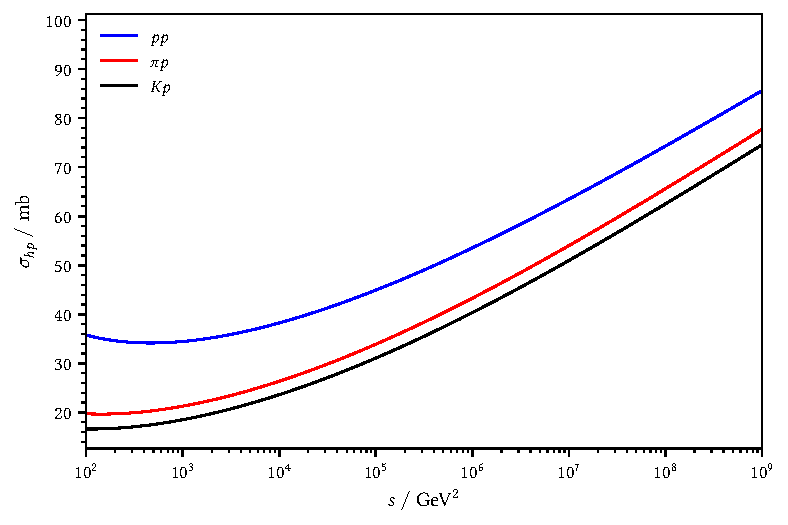
\includegraphics{../plots/build/hadron_proton_scattering.pdf}
	\caption[Inelastic cross sections $\sigma_{h \kern-0.1pt p}$ for hadron-{\kern+0.1pt}proton scattering.]
			{Inelastic cross sections $\sigma_{h \kern-0.1pt p}$ for hadron-{\kern+0.1pt}proton scattering according to the
			 parametrizations \eqref{eqn:hpr1r2} and \eqref{eqn:ratio} reproducing an asymptotic $\cramped{ln^2(s)}$ scaling.}
	\label{fig:hadron-proton-scattering}
\end{figure}




\subsection{Production}
\label{sub:production}

For charm quark production in proton-{\kern+0.1pt}air collisions, reference \cite{Goncalves_2007} gives
\begin{equation*}
	x_F \kern+1.0pt \frac{\raisebox{-0.5ex}{$d\sigma$}}{\raisebox{0.5ex}{$dx_F$}} \bigl( x_F \kern+0.5pt, \kern-0.5pt E_p \bigr)
	\kern-0.1pt = a \kern+0.5pt x_F^b \kern+1.0pt \bigl( 1 \kern-0.3pt - x_F^m \kern+0.3pt \bigr)^n
\end{equation*}
as the parametrized differential cross section with components
\begin{align*}
	a = a_1 \kern-0.5pt \ln\bigl(E_p\bigr) - \kern+0.5pt a_2 && b = b_1 \kern-1.0pt - b_2 \ln\bigl(E_p\bigr) &&
	n = n_1 \kern-1.0pt - \kern+0.5pt n_2 \ln\bigl(E_p\bigr)
\end{align*}
for which table \ref{tab:charm-production} lists all necessary constants. Here, proton energies $E_p$ are defined as viewed
by air nuclei at rest, while the Feynman scaling variable $x_F \kern+1.0pt = p_c \kern+1.5pt / \kern-0.5pt p_s$ specifies
magnitude ratios of produced charm quark longitudinal momentum to all available momentum in center mass coordinates of the
colliding particles. Application of section \ref{sub:frames} shows that this approximately fulfills $x_F \kern+1.0pt = x_c$
where $x_c = \kern+0.2pt E_c \kern+1.0pt / E_p$ in the relevant energy ranges. It should be noted that for the values
table \ref{tab:charm-production} provides, the coefficient $n_0 \kern-0.5pt = \num{0.075}$ from table 1 in \cite{Goncalves_2007} 
for the lower energy regime is set to $n_0 \kern-0.5pt = \num{7.5}$ instead, because the parametrization breaks down otherwise.
Further testing reveals another problem in the \qty{e4}{\giga\electronvolt} to \qty{e8}{\giga\electronvolt} region,
namely that energies around the \qty{26}{\tera\electronvolt} mark or lower result in negative differential cross
sections. Considering other approximation made for this work, it is decided that the
\qty{e8}{\giga\electronvolt} to $10^{1 \kern-0.3pt 1} \kern+1.5pt \unit{\giga\electronvolt}$ case can be extrapolated to all
energies without producing unreasonably large errors. With this choice, the threshold below which unphysical values are
produced is only \qty{140}{\giga\electronvolt} instead, which is well outside the relevant energy ranges.

\begin{table}[H]
	\centering
	\vspace{1.5ex}
	\caption[Parametrization of the $c$ quark differential cross section.]
			{Parametrization of the weighted charm quark
			 production differential cross section. Coefficients are calculated from \cite{Goncalves_2007} to write $E_p$
			 in units of \unit{\giga\electronvolt} without needing redundant conversion steps. The exponent $m = \kern-0.5pt \num{1.2}$
			 is a constant at all energies. For the application at hand, energy ranges beyond the given validity intervals
			 are used as mentioned in the text.}
	\label{tab:charm-production}
	\sisetup{group-digits=integer, table-format=1.3}
	\begin{tabular}{l S[table-format=3.0] S[table-format=4.0] S S S S}
		\midrule\midrule
		{$E_p \mathbin{/} \unit{\giga\electronvolt}$} & {$a_1 \mathbin{/} \unit{\micro\barn}$} &
		{$a_2  \mathbin{/} \unit{\micro\barn}$} & {$b_1$} & {$b_2$} & {$n_1$} & {$n_2$} \\
		\midrule
		{$10^4 - 10^8$} & 826 & 8411 & 0.197 & 0.016 & 8.486 & 0.107 \\
		{$10^8 - 10^{1 \kern-0.3pt 1}$} & 403 & 2002 & 0.237 & 0.023 & 7.639 & 0.102 \\
		\midrule\midrule
	\end{tabular}
\end{table}


As in \cite{Bhattacharya_2015} it is assumed that the cross section scales linearly with nucleon number, yielding
\begin{equation*}
	\frac{\raisebox{-0.5ex}{$d\sigma$}}{\raisebox{0.5ex}{$dx_c$}} \bigl( x_c \kern+0.5pt, \kern-0.5pt E_p \bigr) = A^{-1}
	\frac{\raisebox{-0.5ex}{$d\sigma$}}{\raisebox{0.5ex}{$dx_F$}} \bigl( x_c \kern+0.5pt, \kern-0.5pt E_p \bigr)
\end{equation*}
for inclusive charm production in proton proton collisions. Approximating air as a gas mixture of roughly \qty{75}{\percent}
nitrogen and \qty{25}{\percent} oxygen, one finds $A = \kern-0.3pt \num{14.5}$ for this scaling. Translation of charm quarks
to charmed hadrons is achieved with a folding integral
\begin{equation}
	\frac{\raisebox{-0.5ex}{$d\sigma$}}{\raisebox{0.5ex}{$dx_h$}}
	\bigl( x_h \kern+0.5pt, \kern-0.5pt E_p \bigr) = \int_{\kern+0.5pt x_h}^1 dz \, z^{-1}
	\frac{\raisebox{-0.5ex}{$d\sigma$}}{\raisebox{0.5ex}{$dx_c$}}
	\bigl( x_c \kern+0.5pt, \kern-0.5pt E_p \bigr) \kern+1.0pt D^{\kern+0.5pt h}_c (z)
	\label{eqn:differential}
\end{equation}
where $z = E_h \kern+1.0pt / E_c \kern+0.5pt$ and $x_h = E_h \kern+1.0pt / E_p \kern+0.5pt$ as well as
$x_c = x_h \kern+1.0pt / z$ are fractional energies. Limits for the integration follow from a basic inequality
$E_h \leq E_c \kern+0.2pt \leq E_p$ to incorporate kinematic constraints. Furthermore, the probability
of observing any final state $h$ originating from a $c$ quark is encoded in a \emph{Frag$\kern-0.3pt$mentation Function}
(\abbrev{FF}) $D^{\kern+0.5pt h}_c (z)$ dependent on the fraction of hadron to charm energy. Reference
\cite{Metz_2016} addresses the connection between this concept and that of a \emph{Parton Distribution Function}
(\abbrev{PDF}) among other things. 

Where a \abbrev{PDF} represents the probability density of finding a parton with given momentum in a color neutral particle,
probabilities for color neutral states existing inside individual partons are given by the appropriate \abbrev{FF} instead.
The partons described here are either quarks or gluons, which can be free only asymptotically at high energies due to carrying
color charges. In this limit, the running coupling of \abbrev{QCD} is small enough for a power series expansion to be a sensible
approach, leading to the definition of terms such as \abbrev{LO} and \abbrev{NLO} in reference to exponent order. There exist
different factorization methods to separate these parts from the nonperturbative contributions contained in any \abbrev{PDF} and
\abbrev{FF} for the confined constituents of hadrons. By fitting to existing data or perturbative results, models can extrapolate to
low momentum fractions that have not yet been probed experimentally. A similar procedure has lead \cite{Kniehl_2006} to obtain
\begin{equation}
	D^{\kern+0.5pt h}_{c}(z) = \frac{N_h z \kern+1.0pt (1 - z)^{\kern+0.5pt 2}}
	{\bigl((1 - z)^{\kern+0.5pt 2} + \epsilon_h z \bigl)^{\raisebox{-1.5ex}{$^2$}}}
	\label{eqn:fragmentation}
\end{equation}
with parameters from $\kern+0.5pt e^+e^- \kern-0.8pt$ data in table \ref{tab:charm-hadrons} as the charm hadron \abbrev{FF} used
throughout this work. It is important to note that such functions are invariant under charge conjugation, so that there is no
differentiation between quark to particle or antiquark to antiparticle processes.

% \begin{figure}[H]
% 	\centering
% 	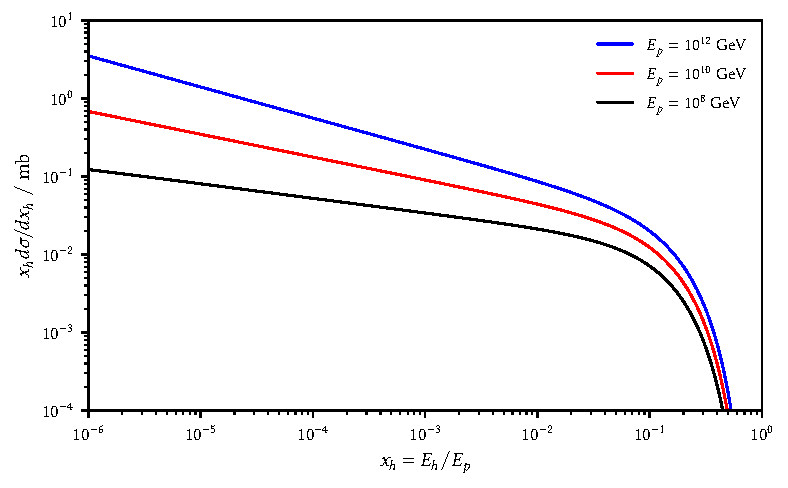
\includegraphics{../plots/build/charm_hadron_cross_section.pdf}
% 	\caption[Inclusive differential cross sections for $\smash{p \kern-0.1pt p \kern+0.6pt \rightarrow D^0 X \kern+0.5pt}$ production.]
% 			{Inclusive differential cross sections for $\smash{p \kern-0.1pt p \kern+0.6pt \rightarrow D^0 X \kern+0.5pt}$ production at
% 			 different proton energies $E_p$ according to the \eqref{eqn:differential} parametrization.}
% 	\label{fig:charm-hadron-cross-section}
% \end{figure}




\section{Spectral Distributions}
\label{sec:spectral}

Constructing spectra $dN_h \kern+0.5pt / dE_h$ from proton injection requires folding of $F_{p \kern+0.8pt \rightarrow h}$ as
the hadronic distribution for a single $p \kern-0.1pt p \kern+0.9pt$ interaction with the number of protons per energy interval
given by the function $dN_p \kern+0.6pt / dE_p$ obtained from source specific modelling. An analogous approach can be applied to
compute neutrino spectra $dN_\nu \kern+0.6pt / dE_\nu$ from $dN_h \kern+0.5pt / dE_h$ via distributions
$F_{\kern+1.0pt h \kern+0.2pt \rightarrow \nu}$ formulated according to the involved decay modes.



\subsection{Charm}
\label{sub:charm}

Spectral distributions for charmed hadron production are calculated according to \cite{Carpio_2020} through
\begin{equation*}
	F_{p \kern+0.8pt \rightarrow h} \bigl( E_h \kern+0.5pt , \kern-0.5pt E_p \bigr) =
	E_p^{\kern+0.5pt -1} \sigma_{p \kern-0.1pt p}^{-1} \bigl( E_p \bigr) \kern+1.0pt
	\frac{\raisebox{-0.5ex}{$d\sigma$}}{\raisebox{0.5ex}{$dx_h$}} \bigl( x_h \kern+0.5pt, \kern-0.5pt E_p \bigr)
\end{equation*}
with $E_h \kern-0.2pt = x_h E_p$ translating between variables. This formula can be understood as a normalization of
\eqref{eqn:differential} against proton energies and the inelastic $p \kern-0.1pt p \kern+0.9pt$ cross section from appendix
\ref{sec:cross} to yield hadron numbers per unit energy.

To find neutrino spectra from charmed hadrons, the same approach as in \cite{Carpio_2020} is used, which assumes an effective
energy distribution approximated by three body decays for the semileptonic channel to a less massive pseudoscalar meson.
By neglecting lepton masses, one obtains
\begin{equation*}
	\tilde{F}_{\kern+1.0pt h \kern+0.2pt \rightarrow \nu \kern+1.0pt} (y) = D_h^{-1} \kern+1.0pt \Bigl( 6b_ha_h^2 - 4a_h^3
	- 12\lambda_h^3 a_h + 12\lambda_h^2 y - 6b_h y^2 + 4 y^3 + 12 \lambda_h^2 \ln \bigl((1 - y) / \lambda_h \bigr) \Bigr)
\end{equation*}
as a distribution with $y = E_\nu \kern+0.6pt / E_h$ and $F_{\kern+1.0pt h \kern+0.2pt \rightarrow \nu \kern+1.0pt}
\bigl( E_\nu \kern+1.0pt , \kern-0.5pt E_h \bigr) = \mathscr{F}_h \tilde{F}_{\kern+1.0pt h \kern+0.2pt \rightarrow \nu \kern+1.0pt}
(y) / E_h$ for conversion.

Hadron specific coefficients for this equation are defined with the parameter
$\lambda_h = \kern+0.5pt \tilde{s}_h / m_h^2 \kern+0.2pt$ as
\begin{align*}
	a_h = 1 - \lambda_h && b_h = 1 - 2\lambda_h &&
	D_h = 1 - 8 \lambda_h - 12\lambda_h^2 \ln \bigl( \lambda_h \bigr) + 8 \lambda_h^3 - \lambda_h^4
\end{align*}
where both $s_h$ and $m_h$ are listed in table \ref{tab:charm-hadrons} for all included charmed hadrons. The assumption of three
body decays like $D^+ \kern-2.5pt \rightarrow \kern+1.0pt \overline{\kern-1.5pt K \kern+1.0pt}\kern+1.0pt^0 e^+ \nu_e$ can
be justified by consulting \cite{pdg} for information on the relevant particles and comparing branching ratios, which indicate
that purely leptonic modes are strongly suppressed. Hadronic channels such as $D^+ \kern-2.5pt \rightarrow \pi^+ \pi^0$ or
$D^+ \kern-2.5pt \rightarrow K^{\kern+0.5pt -} \pi^+ \pi^+$ are either very improbable as well or occur at significant rates but
do not contribute many high energy neutrinos due to pions and kaons being subject to further cooling before decaying to leptons.
By the same logic, secondary muon decay is neglected when determining the neutrino spectrum.

\begin{table}[H]
	\centering
	\vspace{2.0ex}
	\caption[Coefficients for $c$ hadron production, cooling and decay.]
			{Coefficients for charm hadron production,
			 cooling and decay to neutrinos. All parameters $\epsilon_h$ are taken from leading order QCD fits
			 via the FF as defined and described in \cite{Kniehl_2006} with normalizations $N_h$ given by \cite{Carpio_2020}
			 to rescale the integration of \eqref{eqn:fragmentation} over $[0 \kern+0.5pt , \kern-1.5pt 1]$ to approximately match
			 the fractions $f_h$ provided in \cite{Lisovyi_2016} from measurements. Effective masses $\sqrt{\tilde{s}_h}$ and branching
			 fractions $\mathscr{F}_h$ are determined by \cite{Bugaev_1998} and \cite{Bhattacharya_2016} from fitting decay rates.
			 Mean lifetimes $\tau_h$ and masses $m_h$ are adopted from \cite{pdg} in the particle listings. Mass type
			 quantities use natural units.}
	\label{tab:charm-hadrons}
	\sisetup{group-digits=integer, table-format=1.2}
	\begin{tabular}{c S[table-format=1.4] S[table-format=1.5] S[table-format=4.0] S[table-format=1.3] S S}
		\midrule\midrule
		{$h$} & {$N_h$} & {$\epsilon_h$} & {$\tau_h \mathbin{/} \unit{\femto\second}$} & {$\mathscr{F}_h$} &
		{$\sqrt{\tilde{s}_h} \mathbin{/} \unit{\giga\electronvolt}$} & {$m_h \mathbin{/} \unit{\giga\electronvolt}$} \\
		\midrule
		{$D^{0}$} & 0.577 & 0.101 & 410 & 0.067 & 0.67 & 1.86 \\
		{$D^{+}$} & 0.238 & 0.104 & 1033 & 0.176 & 0.63 & 1.87 \\
		{$D^{+}_{s}$} & 0.0327 & 0.0322 & 501 & 0.065 & 0.84 & 1.97 \\
		{$\Lambda^{\kern-0.5pt +}_{\kern+0.5pt c}$} & 0.0067 & 0.00418 & 203 & 0.045 & 1.27 & 2.29 \\
		\midrule\midrule
	\end{tabular}
\end{table}




\subsection{Pions \& Kaons}
\label{sub:pions}

By parametrizing event generator results, a neutral pion production spectrum of the form
\begin{equation*}
	\tilde{F}_\pi \kern+1.5pt \bigl( x_\pi \kern+0.7pt , \kern-0.5pt E_p \bigr) = 4\alpha B x_\pi^{\alpha - 1}
	\left( \frac{1 - \kern+0.2pt x_\pi^\alpha}{1 + \kern+0.8pt rx_\pi^\alpha (1 - \kern+0.2pt x_\pi^\alpha \kern+1.0pt )}
	\right)^{\kern-1.0pt 4} \left( ( 1 - \kern+0.2pt x_\pi^\alpha \kern+1.0pt )^{-1} +
	\frac{r (1 - \kern+0.2pt 2x_\pi^\alpha \kern+1.0pt )}{1 + \kern+0.8pt rx_\pi^\alpha (1 - \kern+0.2pt x_\pi^\alpha \kern+1.0pt )}
	\right) \left( 1 - \kern+0.3pt \frac{m_\pi}{\raisebox{1pt}{$x_\pi \kern+1.0pt E_p$}} \right)^{\kern-1.0pt 1/2}
\end{equation*}
is found in \cite{Kelner_2006} with $m_\pi = \qty{0.135}{\giga\electronvolt}$ \cite{pdg} translated to natural units and parameters
\begin{align*}
	&&&& B \kern+0.5pt = \tilde{B} + C &&
	\alpha \kern+0.5pt = \frac{\raisebox{-1.5pt}{$\tilde{\alpha}$}}{\displaystyle\sqrt{C \kern+1.5pt}} &&
	r \kern+1.0pt = \frac{\raisebox{-1.5pt}{$\tilde{r}$}}{\displaystyle\sqrt{C \kern+1.5pt}} &&&&
\end{align*}
where a low energy cutoff is enforced via $E_\pi \kern-0.1pt = x_\pi \kern+1.0pt E_p$ in the mass term. From
\begin{equation*}
	C = c_1 \kern-0.5pt - \kern+0.5pt c_2 \ln \bigl( E_p \bigr) + \kern+0.5pt  c_3 \ln^2 \bigl( E_p \bigr)
\end{equation*}
results a dependence on projectile energy for the shape of this distribution.\newpage

Coefficients are specified in table \ref{tab:pion-spectrum} and recalculated for $E_p \kern+0.5pt$ in \unit{\giga\electronvolt}
instead of \unit{\tera\electronvolt} units. Under the assumption of a $\smash{\pi^0} \kern-0.5pt$ cross section approximately
equal to the $\smash{\pi^\pm} \kern-0.5pt$ average and with identical spectra for charged pions, it follows that
$F_\pi = \tilde{F}_\pi \kern+0.5pt / E_p$ should describe pion production regardless of charge reasonably well
for the purpose of this work.

\begin{table}[H]
	\centering
	\vspace{2.0ex}
	\caption[Parametrized spectral distribution for pion production.]{Parametrized spectral distribution for
			 neutral pion production. Factors are taken from \cite{Kelner_2006} and converted to write $E_p$
			 in units of \unit{\giga\electronvolt} for $c_k$ coefficients.}
	\label{tab:pion-spectrum}
	\sisetup{group-digits=integer, table-format=1.3}
	\begin{tabular}{S[table-format=1.2] S[table-format=1.2] S[table-format=1.1] S S S}
		\midrule\midrule
		{$\tilde{B}$} & {$\tilde{\alpha}$} & {$\tilde{r}$} & {$c_1$} & {$c_2$} & {$c_3$} \\
		\midrule
		0.25 & 0.98 & 2.6 & 1.515 & 0.206 & 0.075 \\
		\midrule\midrule
	\end{tabular}
\end{table}


For a convenient formulation of kaon production, references \cite{Lykasov_2021} and \cite{Lykasov_2022} indicate a constant ratio
$\pi / K$ at moderately high energies. Similar fractions are retrieved from multiplicities given in \cite{Koers_2006} and lead to
$F_K \kern+0.5pt / F_\pi = \num{0.12}$ as a simplifying assumption, the validity of which cannot be guaranteed for the application
at hand. Calculations of kaon spectra still employ this approach but are subject to considerable reservations as a result.

Decays of pions and kaons to neutrinos are approximated via the $h \rightarrow \mu^+ \nu_\mu$ two body channel with branching
fractions of $\mathscr{F}_{\kern-0.2pt \pi \kern+0.2pt} = \qty{99.99}{\percent}$ and
$\mathscr{F}_{\kern+0.3pt K \kern+0.2pt} = \qty{63.56}{\percent}$ given in the \cite{pdg}
particle listings. By decaying, muons produced in these processes can significantly impact the neutrino spectrum. Results from
\cite{Carpio_2020} suggest that this is particularly relevant for pions. Muonic three body decays of type
$\mu^- \kern-2.5pt \kern+0.5pt \rightarrow e^- \kern+0.5pt \overline{\kern-0.2pt \nu \kern+0.8pt}_e \nu_\mu$ as well as
cooling factors depend on the polarization of participating leptons due to the nature of weak force coupling. This complicates
computations and is thus omitted in service of restricting the present work to a managable scope, though it should be remembered
as an important caveat for the final results.

The remaining two body decays of ultrarelativistic hadrons $h$ to leptons $l \kern+1.0pt$ obey a distribution
\begin{equation*}
	F_{\kern+1.0pt h \kern+0.2pt \rightarrow l \kern+1.0pt} \bigl( E_l \kern+0.8pt, \kern-0.2pt E_h \bigr) =
	\mathscr{F}_{\kern+0.2pt h \kern+0.2pt} E_h^{\kern+1.0pt -1} \bigl( 1 \kern-0.3pt - \lambda_h \bigr)^{-1}
\end{equation*}
with $m_{\kern+0.5pt \nu} = 0$ and $m_\mu = \qty{0.106}{\giga\electronvolt}$ \cite{pdg} as well as
$\lambda_h \kern-0.3pt = m_\mu^2 \kern+0.5pt / m_h^2$ as a parameter. This formula is the same whether $l = \nu \kern+0.2pt$ or
$l = \kern-0.3pt \mu$ because there is one muon for each neutrino. In addition, kinematic considerations lead to
$E_\mu \kern+0.5pt / E_h > \lambda_h$ and $E_{\kern+0.5pt \nu} \kern+0.5pt / E_h < 1 - \lambda_h$ for integral bounds
$E_\mu < E_h < E_\mu \kern+0.5pt / \lambda_h$ in the case of muons or
$E_{\kern+0.5pt \nu} \kern+0.5pt / \smash{\bigl( 1 - \lambda_h \bigr)} < E_h < E_p$ when considering neutrinos.



\section{Computation}
\label{sec:computation}



\subsection{Proton Injection}
\label{sub:injection}



\subsection{Hadron Production \& Decay}
\label{sub:production}



\section{Implementation}
\label{sec:implementation}

In order to calculate neutrino spectra from hadronic distributions, several integrals have to be computed. Discretizing
this task allows the general case
\begin{align*}
	F(x, y) \kern+1.5pt &= \int_{z_{-}}^{z_{+}} dz \: G(x, z) \, H(z, y) \\
	\intertext{to be rewritten as a Riemann sum. Assuming $G$ and $H$ are integrable over a given interval,}
	F_{ij} \kern+1.8pt &= \sum\nolimits_k D_{kk} \, G_{ik} \, H_{kj}
\end{align*}
converges to the exact solution for sufficiently small steps. Transforming variables
\begin{align*}
	&&&& x \rightarrow x_i && y \rightarrow y_j && z \rightarrow z_k &&&&
\end{align*}
and defining $D_{kk} = z_{k+1} \kern-1.0pt - z_k$ leads to the above notation. It is easily shown how this expression in terms of
indices translates to the product of corresponding matrices
\begin{equation*}
	\bm{F} \kern+0.6pt = \bm{G} \, \bm{D} \, \bm{H}
\end{equation*}
as an equivalent formulation. Here the output $\bm{F} \in \mathbb{R}^{m \times n}$ is obtained from the inputs
$\bm{G} \in \mathbb{R}^{m \times l}$ and $\bm{H} \in \mathbb{R}^{l \times n}$ as well as the square matrix
$\bm{D} \in \mathbb{R}^{l \times l}$ that encodes all step sizes on its diagonal. These results enable a quick and
efficient implementation of the required calculations as program code, where array arithmetic operations can greatly
increase execution speed.\footnote{$\,$In service of reproducability, all implementations can be viewed in
\href{https://github.com/fritzali/bachelor}{this} repository.}
